\chapter{Experiment and Evaluation}
\label{chapter:experiment}
In the study of this thesis, we have considered different statistics of different types of distributions. However, we will limit our experiments in the following two statistics.
\begin{enumerate}
\item Distribution of the capacities $C(a)$ as the fixation $a$ varies as approximated in Theorem \ref{general capacity distribution}. Here $C$ is the average of $C\left(a\right)$ over all possible $a$. It is also the capacity of the ML approximation.
%\item Distribution of $T_a(\phi)$ as the data sample $\phi$ varies for a fixed fixation $a$, with mean and variance as mentioned in Equation \ref{eqn:distribution_of_T_fixed_a_variable_phi} where $C\left(a\right)$ is the capacity of a distribution of size $|Y|$ for a single fixation $a$.
\item The distribution of $T(\phi,a)$ as both the data sample $\phi$ and the fixation $a$ vary randomly. This distribution is approximated in Theorem \ref{theorem: variable fixation}.
\end{enumerate} The objective of the experiments is to check how well the experimental distributions of the above mentioned statistics agree with the theoretical approximations. In case of the experiment for the first statistic mentioned in the above list, we have to compute the capacity of the distribution of the values at the output of the SS trail. It requires to encrypt the whole codebook. Encrypting the whole codebook is impossible for the cipher PRESENT described in Section \ref{section:present}. Because the size of the full codebook for this cipher is $2^{64}$ which is too large to handle with the computational capability that we have. To avoid this problem, we have considered smaller versions of PRESENT called SMALLPRESENT-$[4]$ and SMALLPRERSENT-$[8]$. In principle, they are exactly the same PRESENT we have defined in section \ref{section:present} but with only $4$ and $8$ S-boxes. Specifications of smaller variants of PRESENT can be found in \citep{smalpresent}. However, we have dicussed SMALLPRESENT-$[n]$ in general, in Section \ref{section:smallpresent-n}, for the sake of the continuity of our discussion.

\section{SMALLPRESENT-$[n]$} \label{section:smallpresent-n}
It is a similar SPN as we have discussed in section \ref{section:present}. The differences are, in SMALLPRESENT-$[n]$, the block size is $4n$. And in the sBoxLayer, there are $n$ copies of the same S-box which is used in the original PRESENT. The pLayer is given by the following function $P$. Bit at the position $i$ of the state is moved to bit position $P\left(i\right)$, where
\[ P(i) = \left\{
  \begin{array}{l l}
    n \times i \mod{4n - 1} & \quad \text{for $0 \leq i < 4n -1$}\\
    4n - 1 & \quad \text{for $i = 4n-1$}
  \end{array} \right.\]
We note that for $n = 16$, this is exactly the linear transformation used in PRESENT that we have discussed in \ref{section:present}. Figure \ref{fig:smallpresent_4_player_4bit_trail} and \ref{fig:smallpresent_8_player} shows the pLayer of SMALLPRESENT-$[4]$ and SMALLPRESENT-$[8]$ respectiviely. However, as the block size is  now $4n$, the key scheduling algorithm requires a modification that produces kyes of length $4n$ in every round. It is achieved by considering the $4n$ rightmost bits of the corresponding round key of the originial PRESENT. Which means, there is no modification in the key scheduling algorithm but there is a modification in the bits which are considered as a round key. With these specifications, it is clear that when we set $n=16$, SMALLPRESENT-$[n]$ becomes the PRESENT that we have discussed in Section \ref{section:present} \par \noindent Now as we have defined SMALLPRESENT-$[n]$, we need to find feasible SS trails in the pLayers of them, so that we can use these trails in our experiments. In Section \ref{section:choosing_ssa_trail}, we have discussed the principle of choosing an SS trail from the pLayer of an SPN. Based on this principle, in the rest of the sections of this chapter, we have chosen useful SS trails for both of the SMALLPRESENT-$[4]$ and SMALLPRESENT-$[8]$ . However, we will limit our experiments only for the case of SMALLPRESENT-[$4$]. We are also experimenting on SMALLPRESENT-[$8$] considering sampling without replacement and the result will be published in an upcoming research paper.


\section{SS Trails in SMALLPRESENT-$[n]$}
\subsection{SMALLPRESENT-$[4]$}
In SMALLPRESENT-$[4]$, there are only $4$ S-boxes. That means the block size is $16$ bits.  Figure \ref{fig:smallpresent_4_player_9bit_trail} shows the non-linear layer of SMALLPRESENT-$[4]$. The SS trail mentioned in bold lines has $8$ single bit trails in each of those three S-boxes. However, we have not conducted our experiment based on this trail because there are only a few bits left to obtain a sufficiently large sample for each fixation of those $9$ input bits of the trail. 
\begin{figure}[h!]
    \centering
    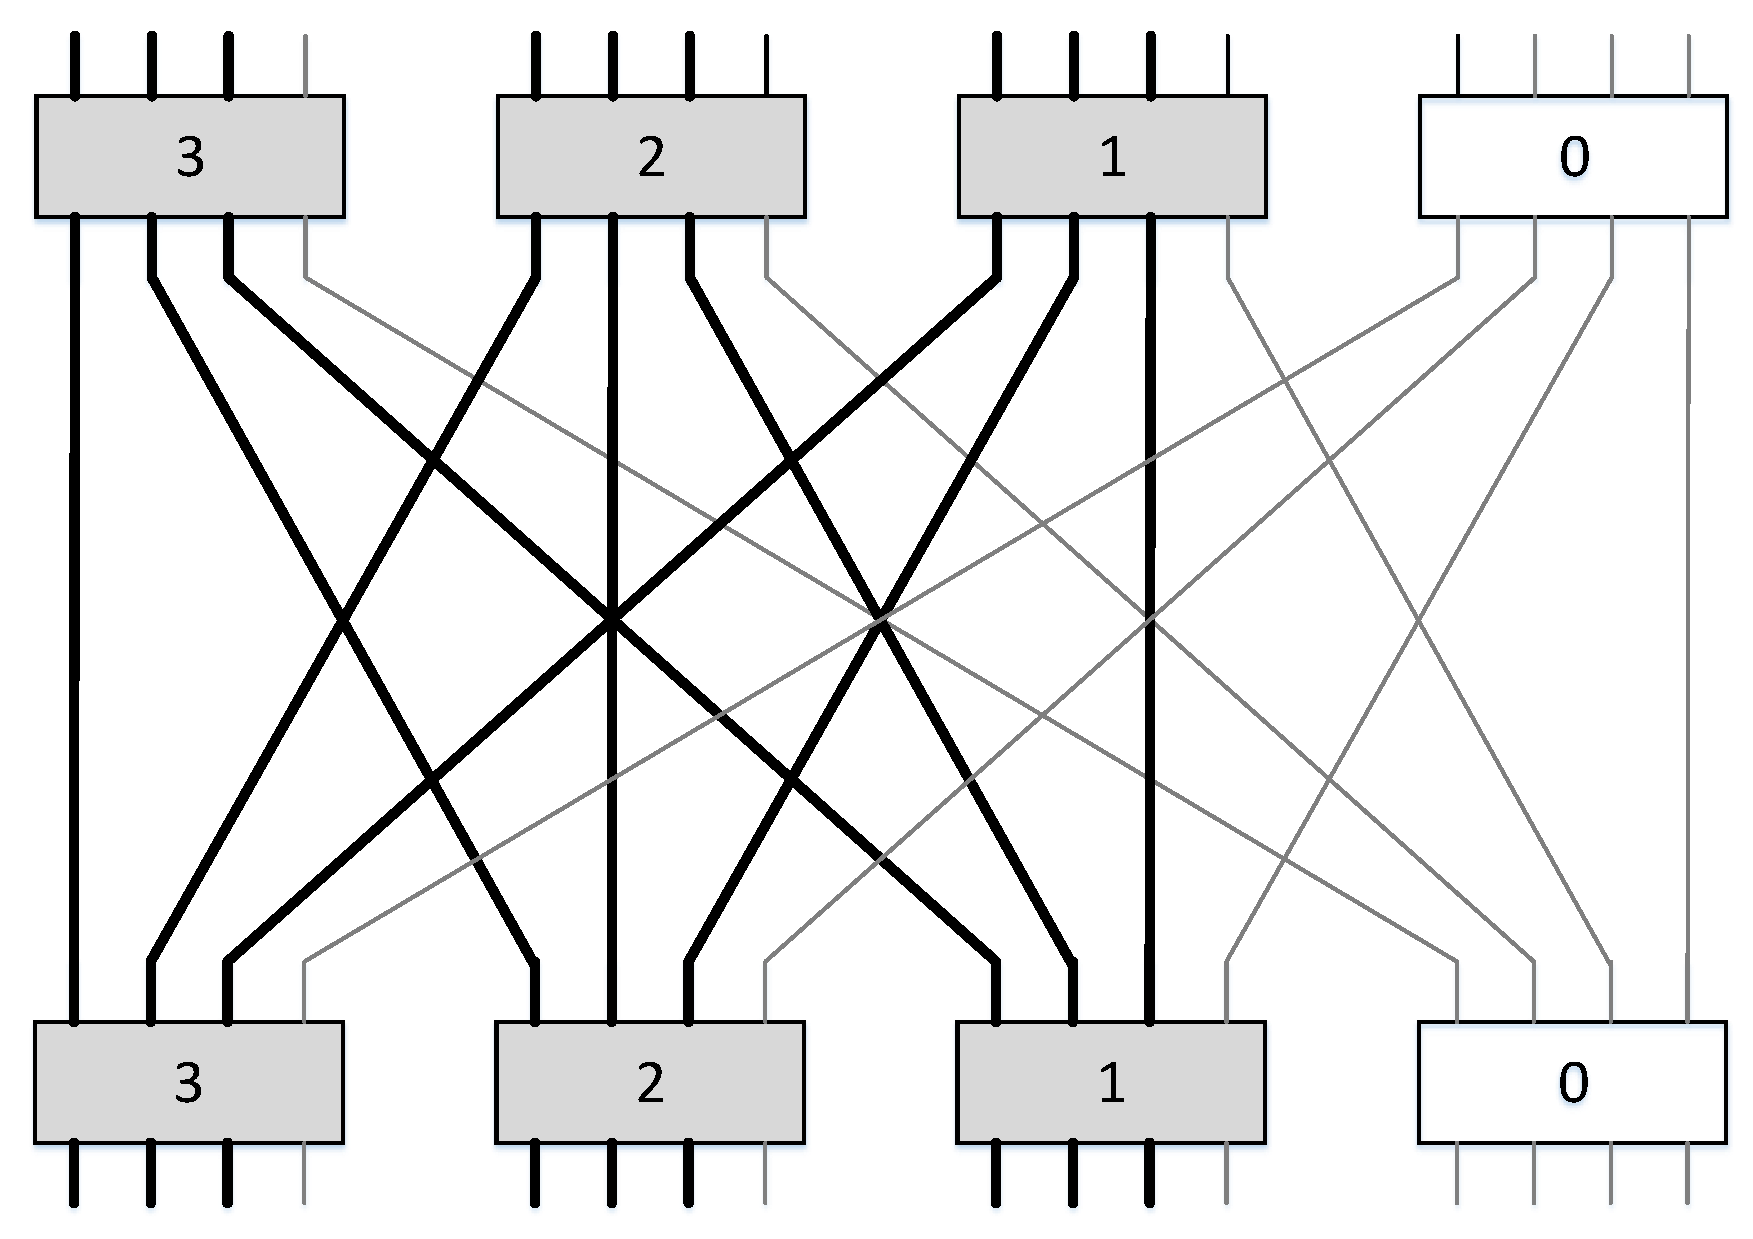
\includegraphics[width=0.9\textwidth,height = 7cm]{images/SMALLPRESENT-4_9bit_trail}
    \caption{9 bit SS trail in SMALLPRESENT-$[4]$.}
    \label{fig:smallpresent_4_player_9bit_trail}
\end{figure}
Fortunately, there is another good trail if we consider the middle two bits of the middle two S-boxes. Because these four bits are involved only among the middle two S-boxes. That is, we have a SS trail of $4$ bits with only $2$ active S-boxes. Figure \ref{fig:smallpresent_4_player_4bit_trail} shows this trail in bold lines. We have used this trail in our experiments later in this chapter.
\begin{figure}[h!]
    \centering
    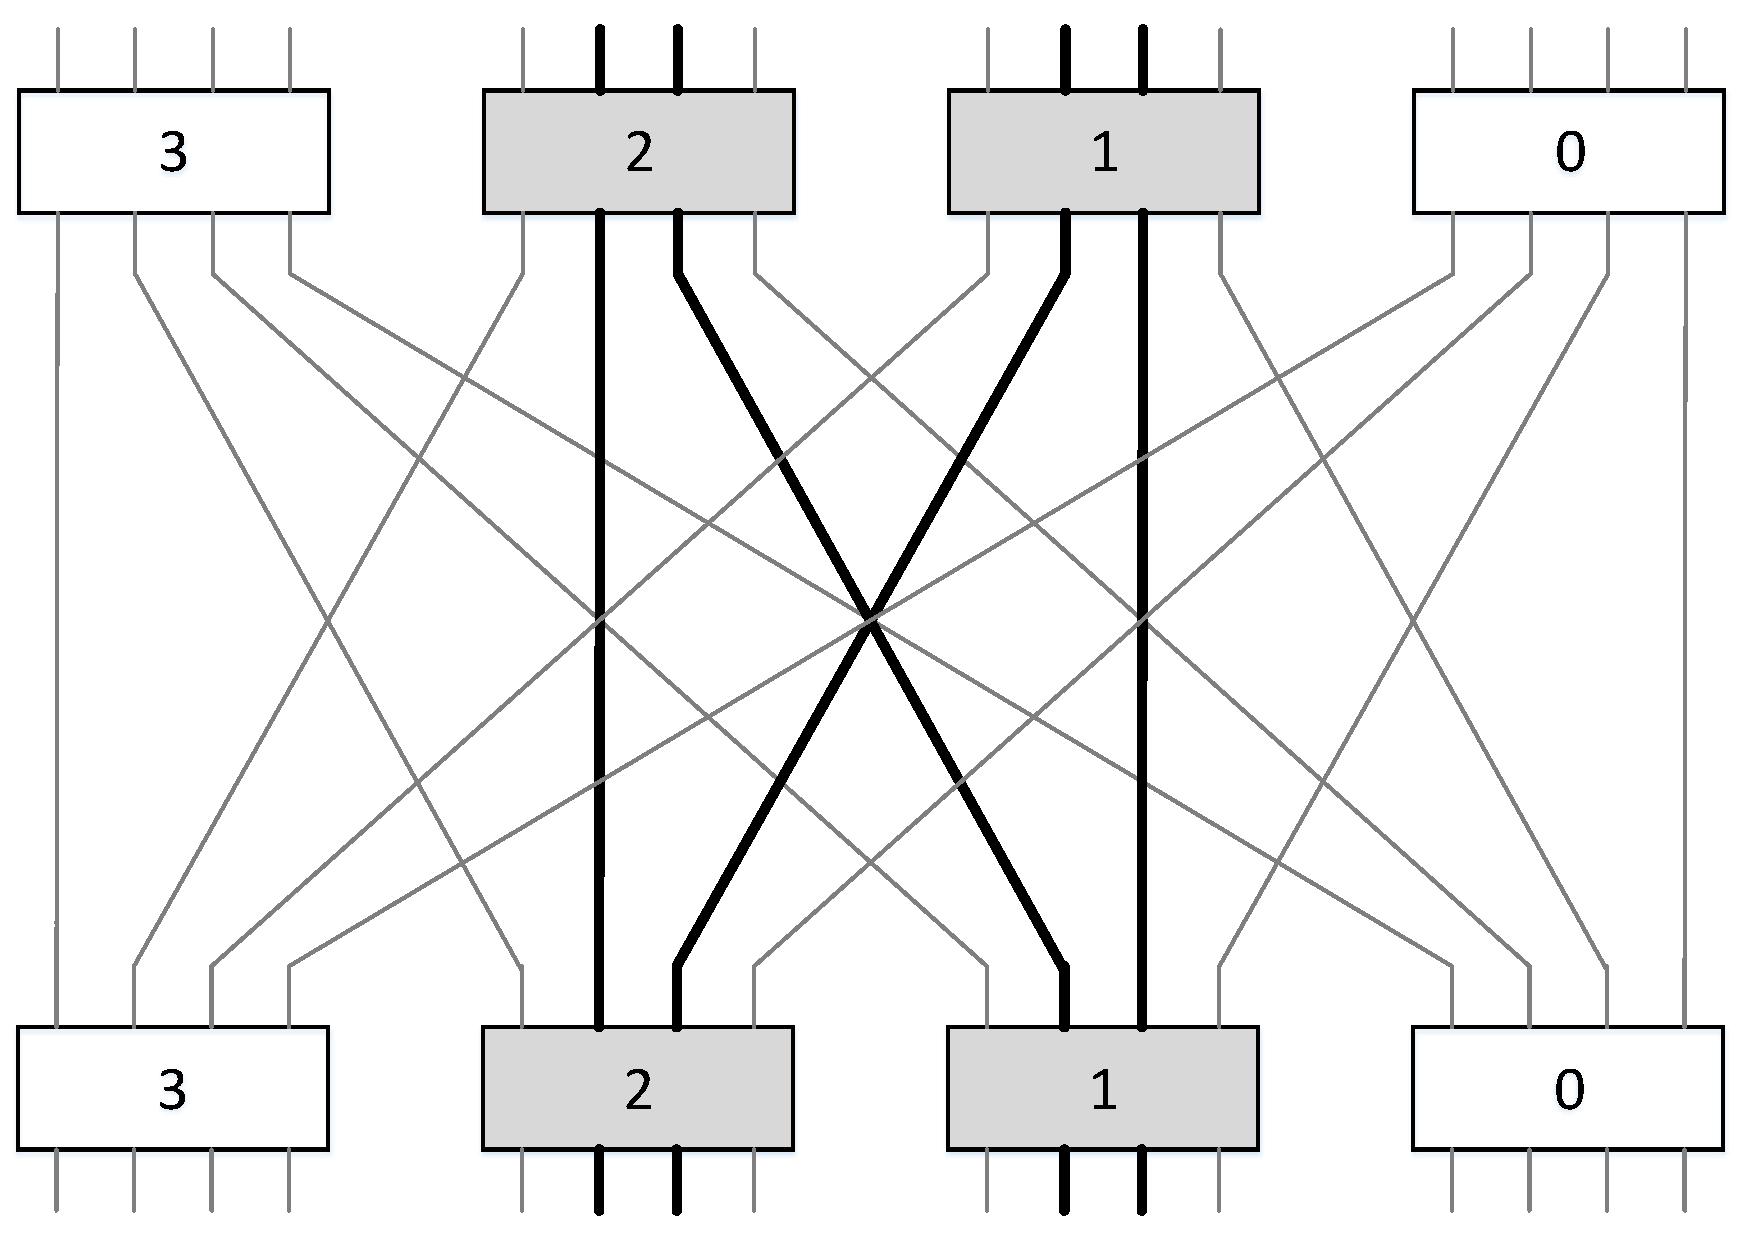
\includegraphics[width=0.9\textwidth,height = 7cm]{images/SMALLPRESENT-4_4bit_trail}
    \caption{4 bit SS trail in SMALLPRESENT-$[4]$.}
    \label{fig:smallpresent_4_player_4bit_trail}
\end{figure}

\subsection{SMALLPRESENT-$[8]$}
In SMALLPRESENT-$[8]$, there are $8$ S-boxes. That means the block size is $32$ bits.   Figure \ref{fig:smallpresent_8_player} shows the non-linear layer of SMALLPRESENT-$[8]$. Based on the principle of choosing an SS trail, we have chosen the trail mentioned in bold lines in this figure. 
\begin{figure}[h!]
    \centering
    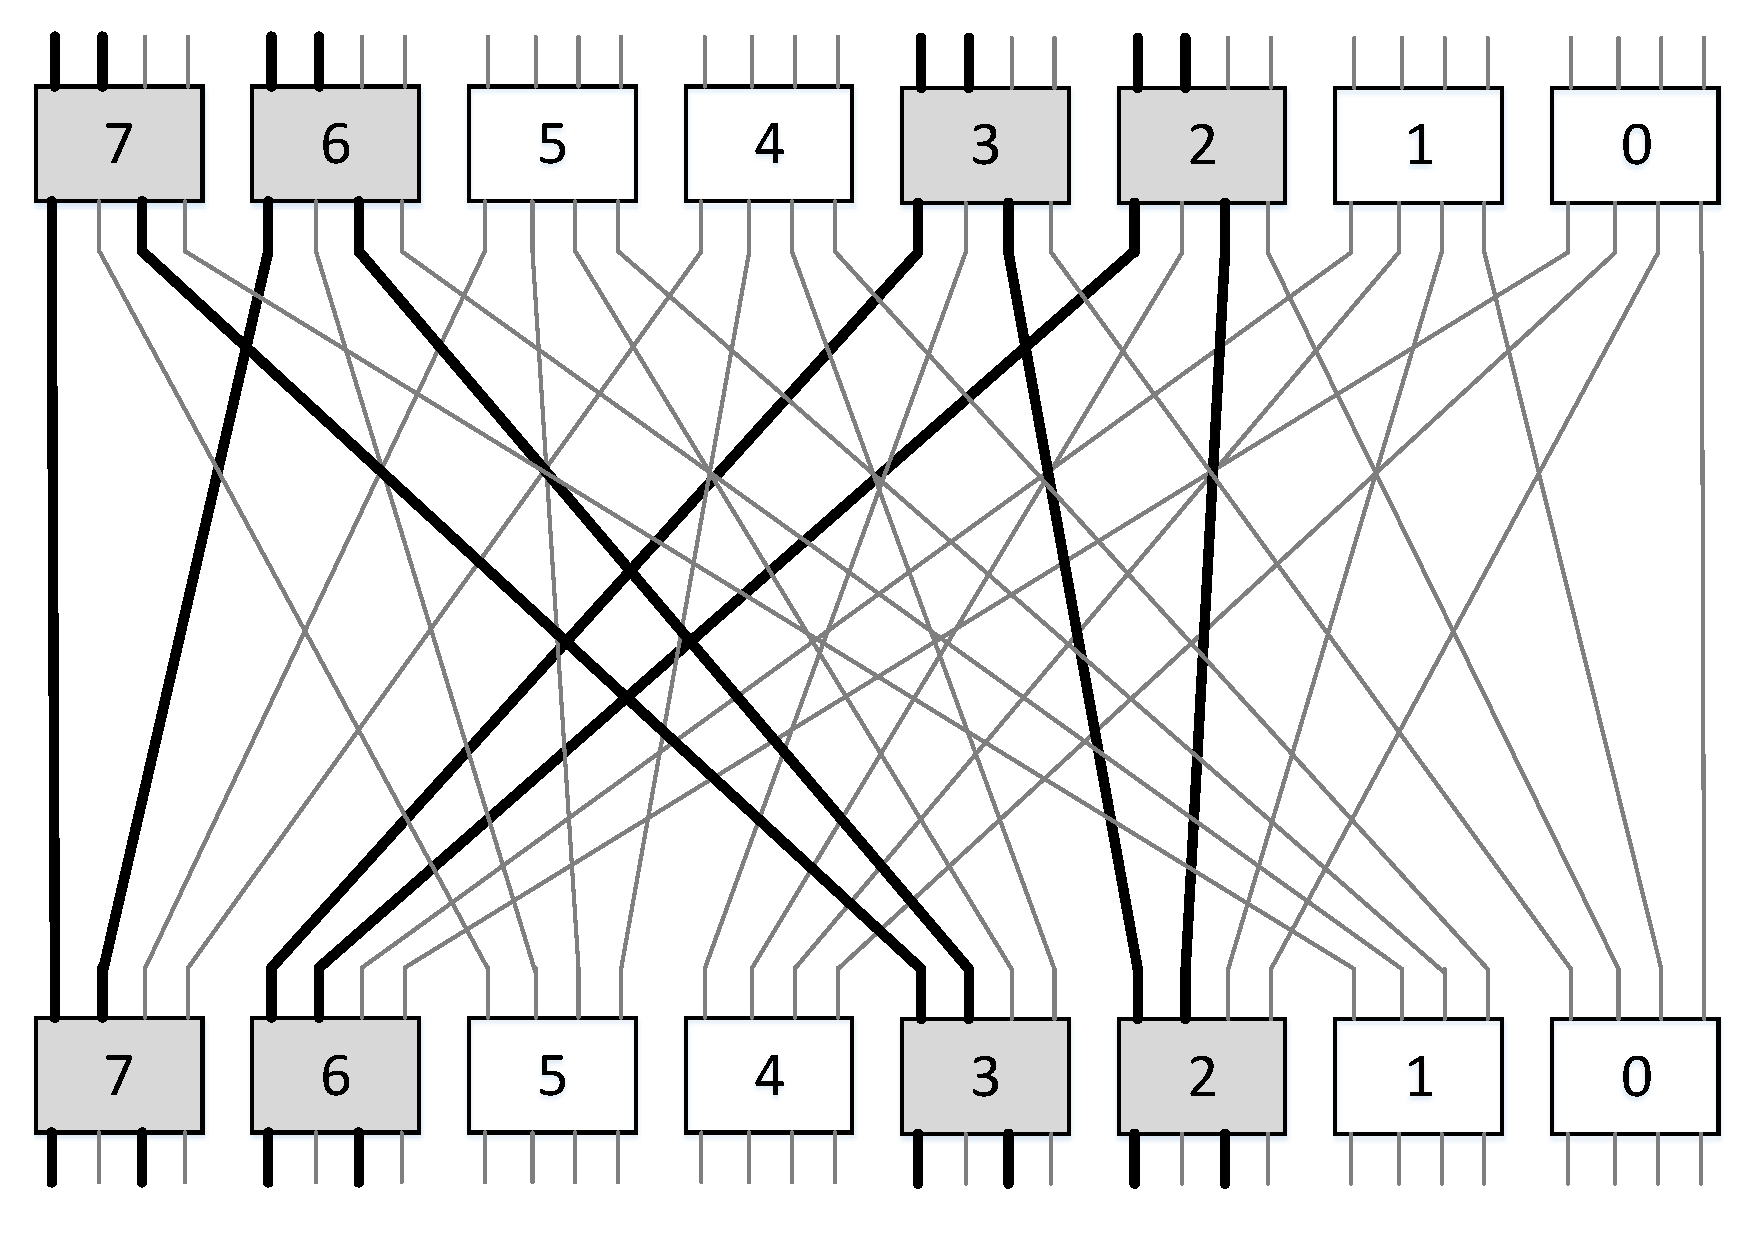
\includegraphics[width=0.9\textwidth,height = 7cm]{images/SMALLPRESENT-8_8bit_trail}
    \caption{8 bit SS trail in SMALLPRESENT-$[8]$.}
    \label{fig:smallpresent_8_player}
\end{figure}
\section{Experiments on SMALLPRESENT-$[4]$}
The trail mentioned in bold lines in Figure \ref{fig:smallpresent_4_player_4bit_trail} is used in these experiments. All the samples that we have used in our experiments are drawn randomly with replacement. At first we investigate the distribution of $C\left(a\right)$ as $a$ varies. As the purpose is to investigate the distribution of $C(a)$, we do not need to consider the key. Then we investigate the distribution of the statistic $T$ for a single fixation where both of the fixation and the sample are varible. Here $a$ is a four bit value, and the size of the distribution is $|Y| = 2^4$.  In the following sections we present the experimental results.
\subsection{SSA Capacities $C(a)$:}
Here $C(a)$ is the capacity of the distribution $p\left(a\right) = \left(p_{\eta}\left(a\right)\right)$ where $a \in \mathbb{F}_2^4$ is the fixation at the input of the trail and $\eta \in \mathbb{F}_2^4$ is the value at the output of the trail. Which means, $C(a)$ is actually $C_{p\left(a\right)}$ as it is defined in Section \ref{section:capacity_of_a_distribution}. And it is computed according to (\ref{eqn:capacity_of_a_distribution}). The experimental value of the variance of $C(a)$ is computed over all the possible fixations $a \in \mathbb{F}_2^4$. The theoretical variance is computed according to Theorem \ref{general capacity distribution}. The result is presented in Table \ref{table:comparing_hypothesis}. \par \noindent From comparative analysis point of view, we observe that, for some numbers of rounds the practical variance is closer to the theoretical one than some other rounds. Now it would be interesting to check how this result agrees with Hypothesis \ref{hyp:hypothesis_on_p_eta_a}. The question is, if the variances of $C(a)$ is  comparatively far from the values predicted by the model, then, is it due to the fact that the probability distributions of $p_{\eta}(a)$ is also far from satisfying the hypothesis? That is, are the variances of  $p_{\eta}(a)$ vary a lot with $\eta$? Similarly, if the variance of $C(a)$ is comparatively closer to the prediction by the model, is it also the case that $p_{\eta}(a)$ have smaller variances? Here $p_{\eta}\left(a\right)$ is calculated using the formula mentioned in (\ref{eqn:p_eta_a}). Which in our case looks like following:
\begin{eqnarray*}
p_{\eta}\left(a\right) = \frac{1}{2^{12}}\left\lbrace x | E_k\left(x,a\right) = \eta  \right\rbrace
\end{eqnarray*}
Table \ref{table:comparing_hypothesis} also compares ``Distance between theoretical and experimental $\sigma^2_{C(a)}$'' with ``variance of $\sigma^2_{p_{\eta}(a)}$ over all $\eta$''
\pagebreak
\begin{center}
\begin{scriptsize}
\captionof{table}{}
\begin{tabular}{l*{4}{c}r} \label{table:comparing_hypothesis}
Round & $C=$ & $\sigma^2_{C(a)}$ &  $\sigma^2_{C(a)}$ & Distance & Variance of $\sigma^2_{p_{\eta}(a)}$ \\
& $\frac{1}{2^4}\sum_{a \in \mathbb{F}_2^4}C(a)$ & (Experimental) & (Theoretical) & & (over all $\eta$)\\
\hline
1 & 1.2500000000 & 0.000000000000 & 0.208333328366 & 0.208333328366 & 0.000000000000000\\
2 & 0.0864257812 & 0.000053644180 & 0.000995922135 & 0.000942277955 & 0.000000000818545\\
3 & 0.0263200998 & 0.000082312916 & 0.000092366354 & 0.000010053438 & 0.000000001487419\\
4 & 0.0084733963 & 0.000012357389 & 0.000009573126 & 0.000002784263 & 0.000000000223686\\
5 & 0.0046606063 & 0.000002714300 & 0.000002896167 & 0.000000181867 & 0.000000000046755\\
6 & 0.0039848089 & 0.000002259238 & 0.000002117160 & 0.000000142078 & 0.000000000014765\\
7 & 0.0029691457 & 0.000000661685 & 0.000001175444 & 0.000000513759 & 0.000000000015007\\
8 & 0.0041698217 & 0.000001235339 & 0.000002318322 & 0.000001082983 & 0.000000000019639\\
9 & 0.0041134357 & 0.000002544029 & 0.000002256047 & 0.000000287982 & 0.000000000015644\\
10 & 0.0029462575 & 0.000001245313 & 0.000001157391 & 0.000000087922 & 0.000000000024034\\
11 & 0.0030920505 & 0.000000583181 & 0.000001274770 & 0.000000691590 & 0.000000000015651\\
12 & 0.0034888982 & 0.000002455807 & 0.000001622988 & 0.000000832819 & 0.000000000030971\\
13 & 0.0038551092 & 0.000001477955 & 0.000001981582 & 0.000000503627 & 0.000000000017599\\
14 & 0.0035421848 & 0.000001178269 & 0.000001672943 & 0.000000494674 & 0.000000000022411\\
15 & 0.0033624172 & 0.000001049226 & 0.000001507447 & 0.000000458220 & 0.000000000015530\\
16 & 0.0040042400 & 0.000001861589 & 0.000002137858 & 0.000000276270 & 0.000000000012828\\
17 & 0.0033563375 & 0.000000747953 & 0.000001502000 & 0.000000754047 & 0.000000000013699\\
18 & 0.0033963918 & 0.000001104406 & 0.000001538064 & 0.000000433658 & 0.000000000016437\\
19 & 0.0035276412 & 0.000001275685 & 0.000001659234 & 0.000000383549 & 0.000000000009210\\
20 & 0.0036349296 & 0.000002631222 & 0.000001761695 & 0.000000869527 & 0.000000000026018\\
21 & 0.0034182071 & 0.000001446692 & 0.000001557885 & 0.000000111193 & 0.000000000017467\\
22 & 0.0035172700 & 0.000004566781 & 0.000001649492 & 0.000002917289 & 0.000000000038211\\
23 & 0.0029666423 & 0.000001265739 & 0.000001173462 & 0.000000092277 & 0.000000000009836\\
24 & 0.0026813745 & 0.000000865261 & 0.000000958636 & 0.000000093375 & 0.000000000012813\\
25 & 0.0035705566 & 0.000002094620 & 0.000001699850 & 0.000000394770 & 0.000000000024349\\
26 & 0.0033077001 & 0.000000503365 & 0.000001458784 & 0.000000955419 & 0.000000000018401\\
27 & 0.0032589435 & 0.000001036276 & 0.000001416095 & 0.000000379819 & 0.000000000020941\\
28 & 0.0035127401 & 0.000002022870 & 0.000001645246 & 0.000000377624 & 0.000000000025578\\
29 & 0.0032626390 & 0.000001063931 & 0.000001419308 & 0.000000355377 & 0.000000000015406\\
30 & 0.0038447380 & 0.000002793566 & 0.000001970935 & 0.000000822632 & 0.000000000035005\\
31 & 0.0032460689 & 0.000001083049 & 0.000001404929 & 0.000000321879 & 0.000000000040317\\
\end{tabular}
\end{scriptsize}
\end{center} \par \noindent Comparatively, we find that the theoretical model disagrees strongly in round $22$ but agrees  better in round $23$. And interestingly we find that the variance of $p_{\eta}(a)$ over all $\eta$ in round $22$ is very large but comparatively small in round $23$. This suggests that the smaller the distance between the theoretical model and  the experimental computation, the closer the hypothesis tends to be valid. %In the next section we will check this phenomenon in the case of statistic $T\left(\phi,a\right)$. 
\par \noindent One important thing to note here is that we do not yet have a proper understanding of what is a small difference or what is a large difference in between the theoretical and experimental values. But we know that our objective is to be a able to distinguish a distribution from random. In other words, we need to know, how useful the theoretical models are, when we use them to perform the statistical test. To visualize this effect, let us check how the theoretical and experimental values of the statistic $T\left(\phi,a\right)$ evolves as the sample size grows and when they start to distinguish from the random distribution.

\subsection{Statistic $T\left(\phi,a\right)$}
\iffalse
Here we will be evaluating Theorem \ref{theorem: variable fixation}. In Table \ref{table:T_a_variable_a_variable_phi_full_codebook}, the comparison is done using sample $\phi$ to be all the possible plaintexts with fixation $a$. So, in the current context $\phi = \mathbb{F}_2^{12}$. The sampling of the chosen plaintexts are done randomly without replacement. 
\begin{center}
\begin{scriptsize}
\captionof{table}{}
\begin{tabular}{l*{4}{c}r} \label{table:T_a_variable_a_variable_phi_full_codebook}
Round & $\mu_{T(\phi,a)}$ &  $\mu_{T(\phi,a)}$ & $\sigma^2_{T(\phi,a)}$ & $\sigma^2_{T(\phi,a)}$ & variance of $\sigma^2_{p_{\eta}(a)}$ \\
 & (Experiment) &  (Theory) & (Experiment) & (Theory) & (over all eta) \\
\hline
1 & 5105.4043 & 5105.4043 & 7138.4285 & 3475353.7379 & 0.000000014823301\\
2 & 372.2495 & 372.2495 & 1908.7264 & 18475.9599 & 0.000000000925185\\
3 & 127.3325 & 127.3325 & 2165.3678 & 2161.8094 & 0.000000002349859\\
4 & 46.7144 & 46.7144 & 314.0983 & 290.9641 & 0.000000000356634\\
5 & 36.2334 & 36.2334 & 171.5494 & 175.0479 & 0.000000000122619\\
6 & 29.6890 & 29.6890 & 66.1217 & 117.5246 & 0.000000000153912\\
7 & 26.7393 & 26.7393 & 142.5548 & 95.3317 & 0.000000000047919\\
8 & 31.2900 & 31.2900 & 128.2649 & 130.5422 & 0.000000000063969\\
9 & 31.0596 & 31.0596 & 147.5356 & 128.6263 & 0.000000000096241\\
10 & 26.8184 & 26.8184 & 37.0340 & 95.8966 & 0.000000000020260\\
11 & 32.7720 & 32.7720 & 71.0487 & 143.2003 & 0.000000000123782\\
12 & 28.8843 & 28.8843 & 82.0928 & 111.2402 & 0.000000000048031\\
13 & 27.8760 & 27.8760 & 82.6281 & 103.6093 & 0.000000000042345\\
14 & 28.1372 & 28.1372 & 84.9019 & 105.5603 & 0.000000000134887\\
15 & 27.6509 & 27.6509 & 101.1446 & 101.9428 & 0.000000000067674\\
16 & 31.7510 & 31.7510 & 102.2708 & 134.4166 & 0.000000000101584\\
17 & 24.4453 & 24.4453 & 111.6897 & 79.6764 & 0.000000000074382\\
18 & 34.2988 & 34.2988 & 150.9873 & 156.8546 & 0.000000000061766\\
19 & 32.1738 & 32.1738 & 139.6693 & 138.0207 & 0.000000000097652\\
20 & 28.4150 & 28.4150 & 93.7672 & 107.6553 & 0.000000000041508\\
21 & 28.3413 & 28.3413 & 96.7962 & 107.0973 & 0.000000000059939\\
22 & 31.7378 & 31.7378 & 106.5411 & 134.3050 & 0.000000000098388\\
23 & 28.8462 & 28.8462 & 136.7566 & 110.9470 & 0.000000000100681\\
24 & 27.6494 & 27.6494 & 61.0345 & 101.9320 & 0.000000000070456\\
25 & 27.4243 & 27.4243 & 153.7815 & 100.2791 & 0.000000000087872\\
26 & 27.3394 & 27.3394 & 60.1927 & 99.6587 & 0.000000000067826\\
27 & 30.8081 & 30.8081 & 83.5536 & 126.5519 & 0.000000000085514\\
28 & 28.8550 & 28.8550 & 165.2511 & 111.0147 & 0.000000000076191\\
29 & 30.2554 & 30.2554 & 197.2302 & 122.0517 & 0.000000000106616\\
30 & 30.2812 & 30.2812 & 223.7799 & 122.2605 & 0.000000000095609\\
31 & 27.1299 & 27.1299 & 76.0133 & 98.1374 & 0.000000000121043\\\end{tabular}
\end{scriptsize}
\end{center}
We observe the same phenomenon here also as we observed in Table \ref{table:comparing_hypothesis}. 
\fi
\par \noindent For each fixation $a$ we draw a line for the statistic $T\left(\phi,a\right)$ computed from experimental data. We plot the size of the sample in the $X$-axis. The same sample is used for all the fixations. That is, For all samples $\phi_1,\phi_2$ used in the experiment, if $|\phi_1| = |\phi_2|$, then $\phi_1 = \phi_2$. And if $|\phi_1| < |\phi_2|$, then $\phi_1 \subset \phi_2$. We also draw the lines for variable fixation and variable sample calculated from theoretical distribution as in Theorem \ref{theorem: variable fixation} and presented in gray color. The dark gray area represents $1$ standard deviation around the theoretical mean. And the light gray area represents $2$ standard deviation around the theoretical mean. We draw the plotting for round $3,4,22$ and $23$ in Figures \ref{fig:T_a_phi_variable_a_varible_phi_variable_size_03rounds}, \ref{fig:T_a_phi_variable_a_varible_phi_variable_size_04rounds},\ref{fig:T_a_phi_variable_a_varible_phi_variable_size_22rounds} and \ref{fig:T_a_phi_variable_a_varible_phi_variable_size_23rounds}. The reason to draw the plot of round $3$ and $4$ is to see how the evolution of the statistic happens in case of smaller number of rounds. And round $22$, $23$ are chosen as they were found interesting in previous section. Observe that, in all the cases of round $3,4,22$ and $23$, they are in close accordance with the theoretical distribution. And in the cases of round $3$ and $4$, both of the theoretical and experimental distribution distinguishes itself from the uniformly random distribution. \par \noindent These plots are also in close accordance with the theoretical data complexity $N_{SS}$ that we have derived in previous chapter. In practice, distinguishing becomes possible when the sample size is large enough so that all the red lines are clearly above the random ($T = 15$). In theory, we can calculate the estimates of $N_{SS}$ using (\ref{eqn:N_ss}). First we set the values of $\zeta_0 = \zeta_1$ to  $\sqrt{2}$ which theoretically suppose to provide $85\%$ success probability of the statistical test. Then using the values of $C$ for the corresponding round gives the theoretical estimation of $N_{SS}$ for that particular round. We see that using this method the theoretical values of $N_{SS}$ for round $3,4,22$ and $23$ are around $2^{10.20},2^{11.84},2^{13.1}$ and $2^{13.35}$ respectively. In contrast, from the experimental plots we see that the red lines start to distinguish at around the same values of $|\phi|$ in the horizontal axis for the case of round $3$ and $4$. From the theoretical values of $N_{SS}$ for round $22$ and $23$, we also find that it distinguishes at the value of $N_{SS}$ which is larger than the full codebook for a fixation. And this is also visible in the plots of those rounds. They do not distinguish at all.

\begin{figure}[h!]
    \centering
    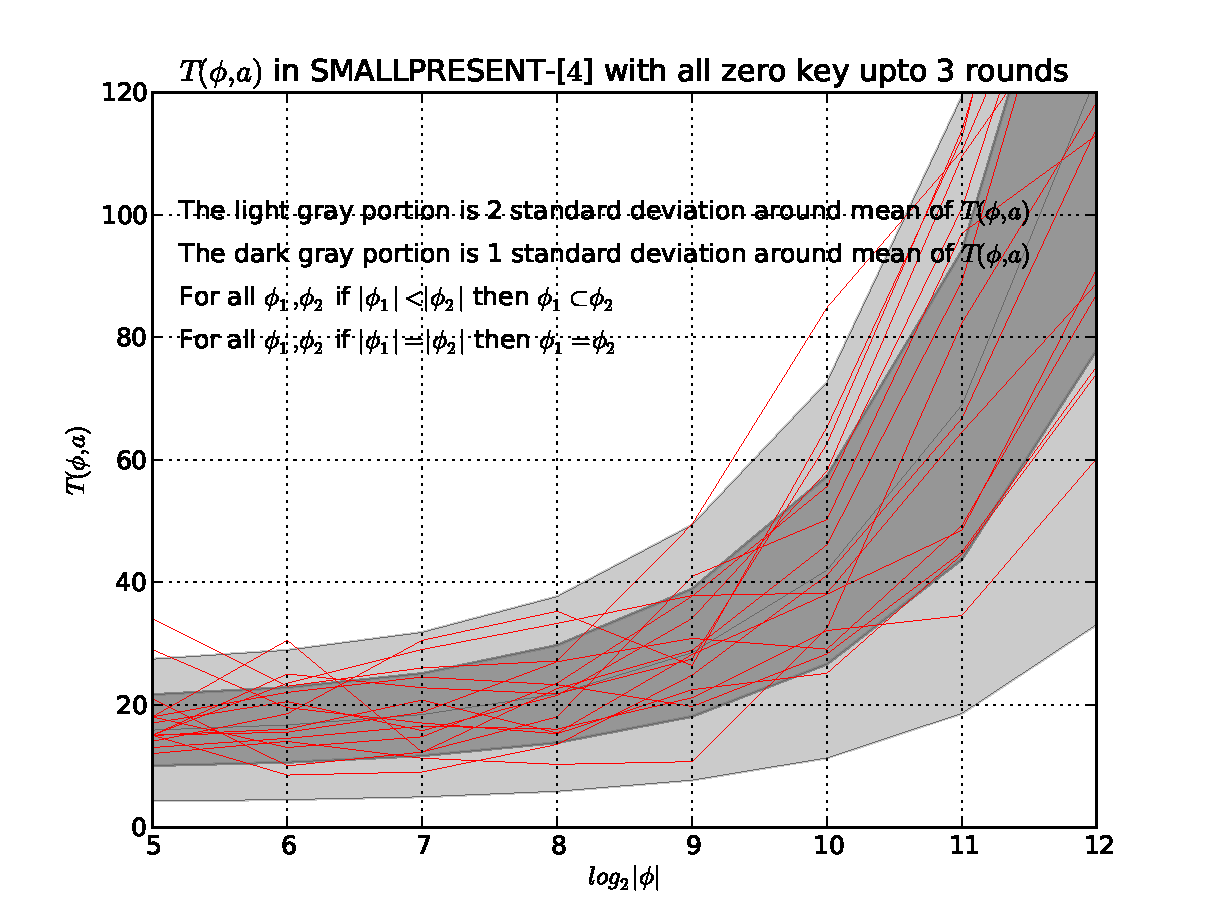
\includegraphics[width=\textwidth , height = 8cm]{images/T_a_phi_variable_a_varible_phi_variable_size_03rounds}
    \caption{$T(\phi,a)$ with $3$ rounds}
    \label{fig:T_a_phi_variable_a_varible_phi_variable_size_03rounds}
\end{figure}

\begin{figure}[h!]
    \centering
    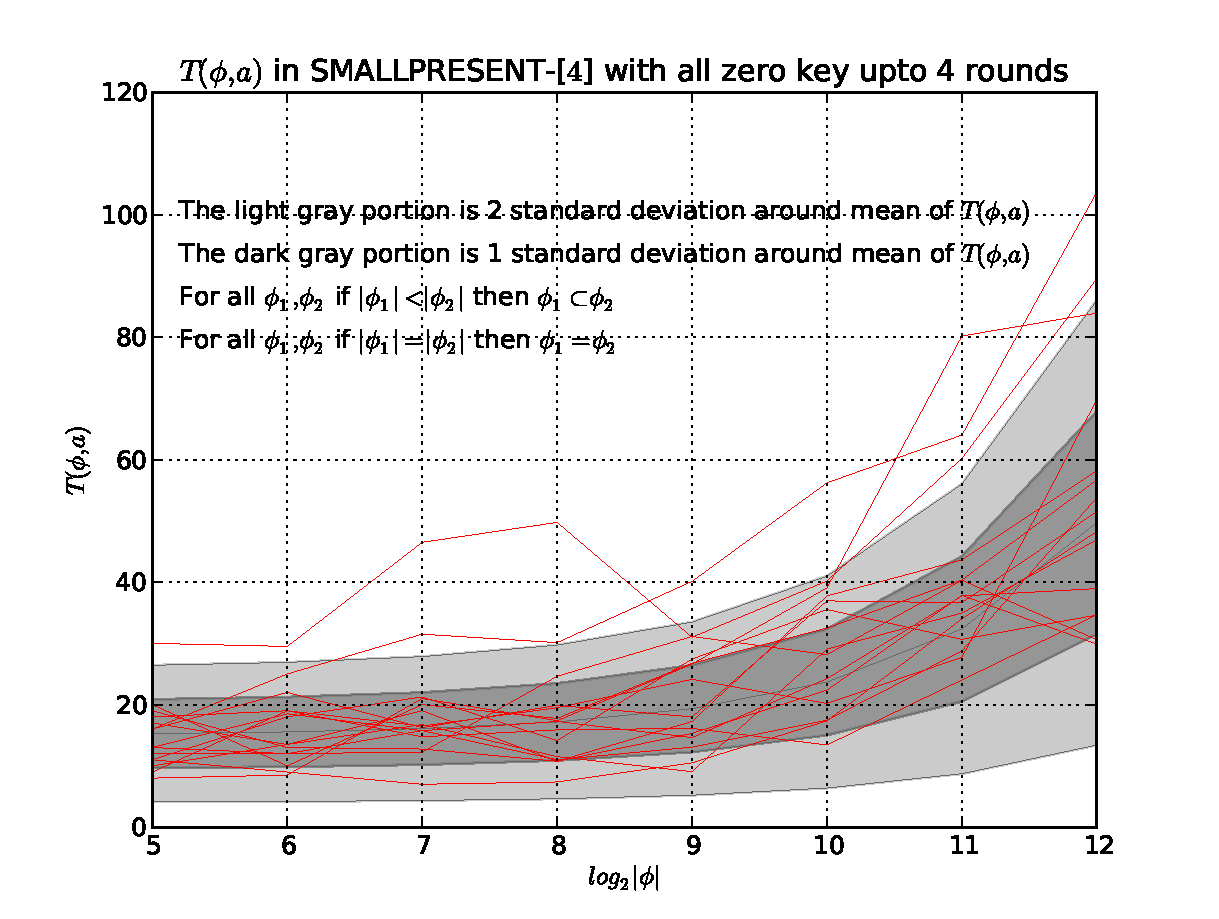
\includegraphics[width=\textwidth , height = 8cm]{images/T_a_phi_variable_a_varible_phi_variable_size_04rounds}
    \caption{$T(\phi,a)$ with $4$ rounds}
    \label{fig:T_a_phi_variable_a_varible_phi_variable_size_04rounds}
\end{figure}

\begin{figure}[h!]
    \centering
    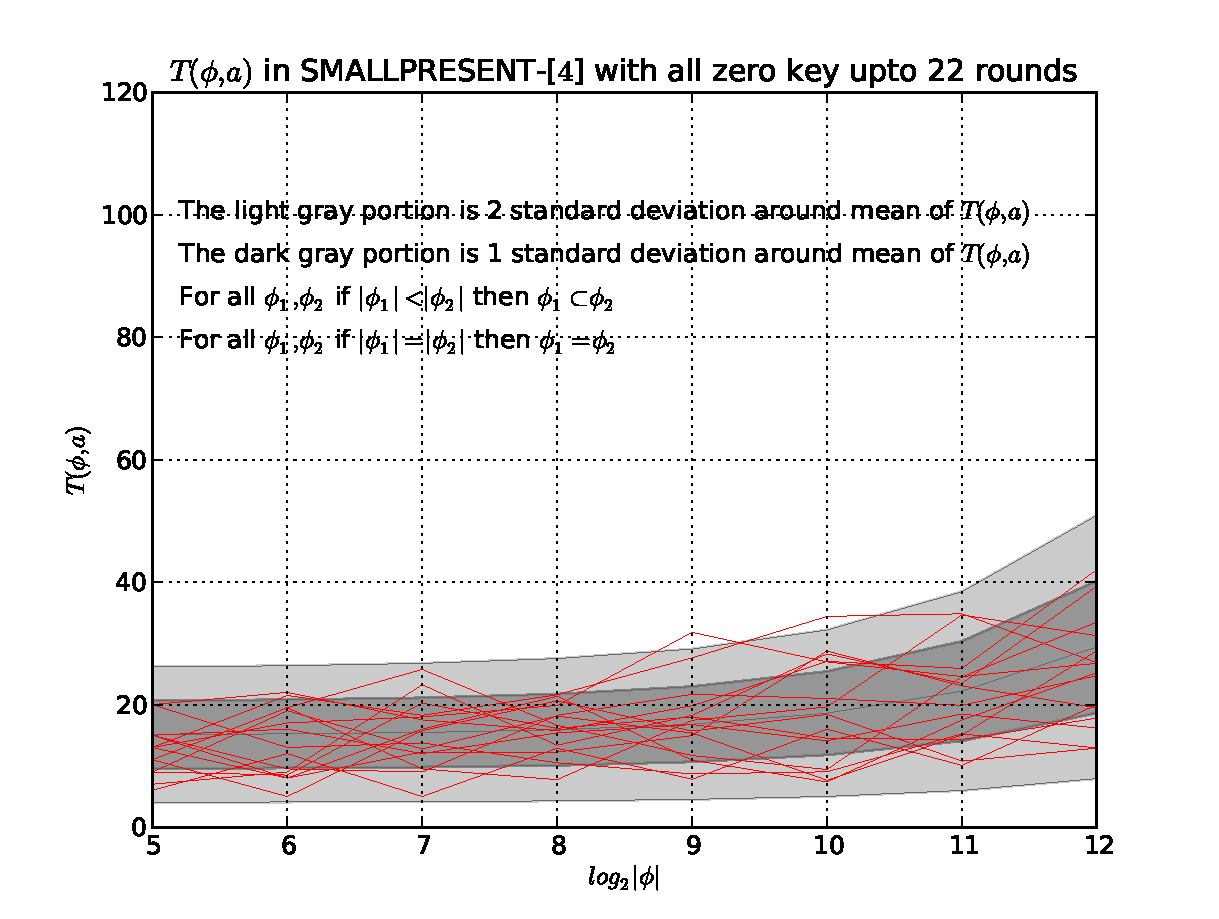
\includegraphics[width=\textwidth , height = 8cm]{images/T_a_phi_variable_a_varible_phi_variable_size_22rounds}
    \caption{$T(\phi,a)$ with $22$ rounds}
    \label{fig:T_a_phi_variable_a_varible_phi_variable_size_22rounds}
\end{figure}

\begin{figure}[h!]
    \centering
    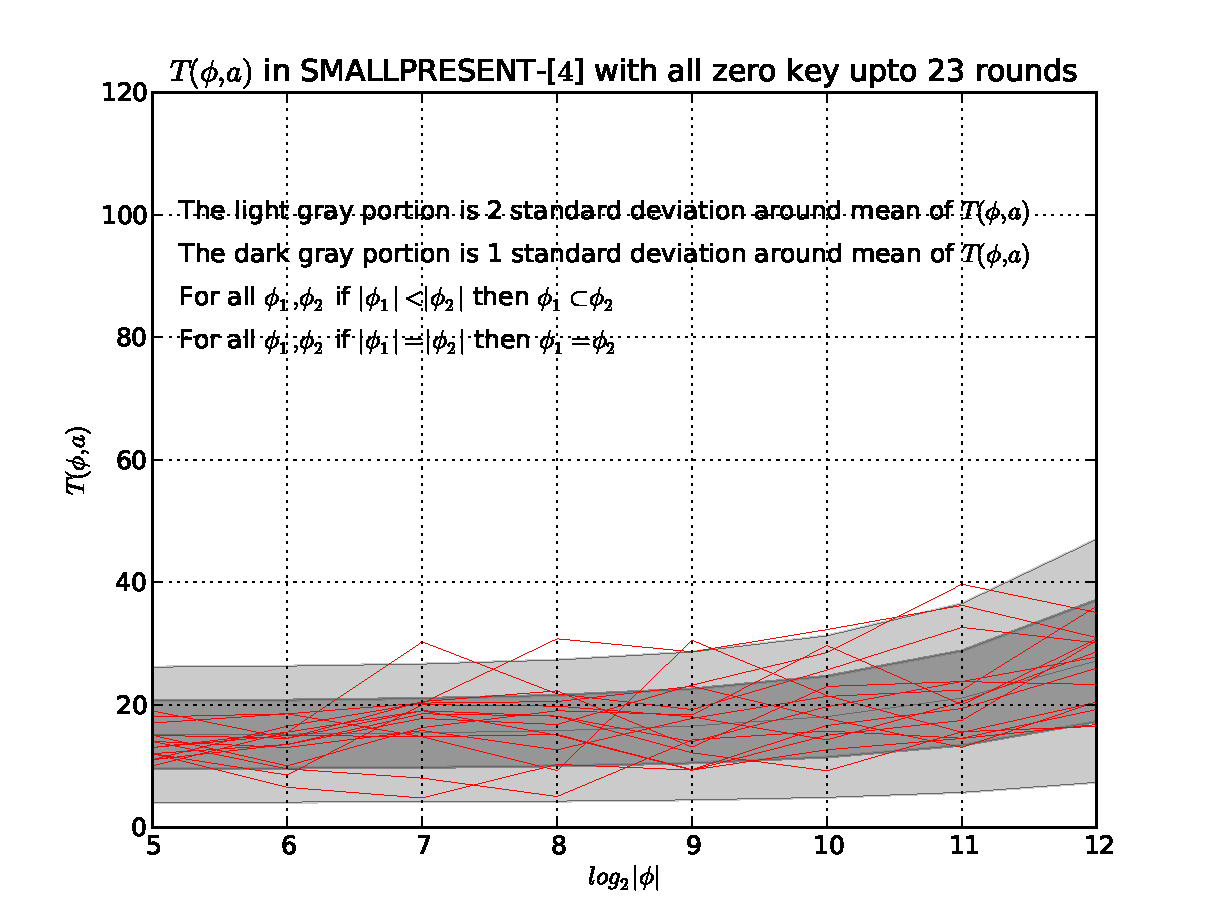
\includegraphics[width=\textwidth , height = 8cm]{images/T_a_phi_variable_a_varible_phi_variable_size_23rounds}
    \caption{$T(\phi,a)$ with $23$ rounds}
    \label{fig:T_a_phi_variable_a_varible_phi_variable_size_23rounds}
\end{figure}%\subsection{Evaluating $T\left(\phi,a\right)$ with $\phi$ sampled randomly with replacement:}
\par \noindent So far, in the experiments of $T\left(\phi,a\right)$, we have used the same sample of equal size for each fixation. Now, let us do the experiment in another way. Let us look at distribution of $T\left(\phi,a\right)$ for a particular round using different fixations and samples of similar sizes. We have used all the possible fixations from 0x0 to 0xf. For each fixation, we have $10000$ samples. Each sample has a size of $2048$ plaintexts and they are chosen randomly with replacement. In this way we had $10000 \times 16 = 160000$ different $T\left(\phi,a\right)$ values. We have calculated the mean and variance of these values of $T$. Then we have compared these with the theoretical values obtained from Theorem \ref{theorem: variable fixation}. Figures \ref{fig:T_a_phi_variable_a_variable_phi_03_round},\ref{fig:T_a_phi_variable_a_variable_phi_04_round},\ref{fig:T_a_phi_variable_a_variable_phi_22_round} and \ref{fig:T_a_phi_variable_a_variable_phi_23_round} shows the theoretical and experimental distribution for round $03,04,22$ and $23$. We observe that the experimental distribution is a little skewed than the theoretical distribution. This is expected as the statistic is originally $\chi^2$ distributed and we have used a normal approximation of $\chi^2$ distribution. As the normal approximation of $\chi^2$ distribution is better satisfied for higher degree of freedom, we understand that the experimental and theoretical distribution will agree better as the number of bits at the output of the SS trail grows. Note that, as like the previous visualization, we observe the same phenomenon in these plots also. For round $3$ it nicely distinguishes from uniform distribution. For round $4$ it looks slightly worse. Nevertheless, it is understandable that the $N_{SS}$ for round $4$ is $2^{11.84}$ and we have used sample of size $2^{11}$ only. And for round $22$ and $23$, they do not distinguishes at all.
\iffalse
\begin{center}
\begin{scriptsize}
\captionof{table}{}
\begin{tabular}{l*{4}{c}r} \label{table:T_a_phi_variable_a_variable_phi}
Round & C & $\mu_{T\left(\phi,a\right)}$ &  $\sigma^2_{T\left(\phi,a\right)}$ & $\mu_{T\left(\phi,a\right)}$ & $\sigma^2_{T\left(\phi,a\right)}$ \\
 & & (Experimental) &  (Experimental) & (Theoretical) & (Theoretical) \\
\hline
15 & 0.003362 & 21.876377 & 61.863674 & 21.885376 & 63.862624355\\
16 & 0.004004 & 23.209412 & 70.374428 & 23.200192 & 71.766521178\\
17 & 0.003356 & 21.855230 & 60.741642 & 21.873088 & 63.790930487
\end{tabular}
\end{scriptsize}
\end{center}
\fi

\begin{figure}[h!]
    \centering
    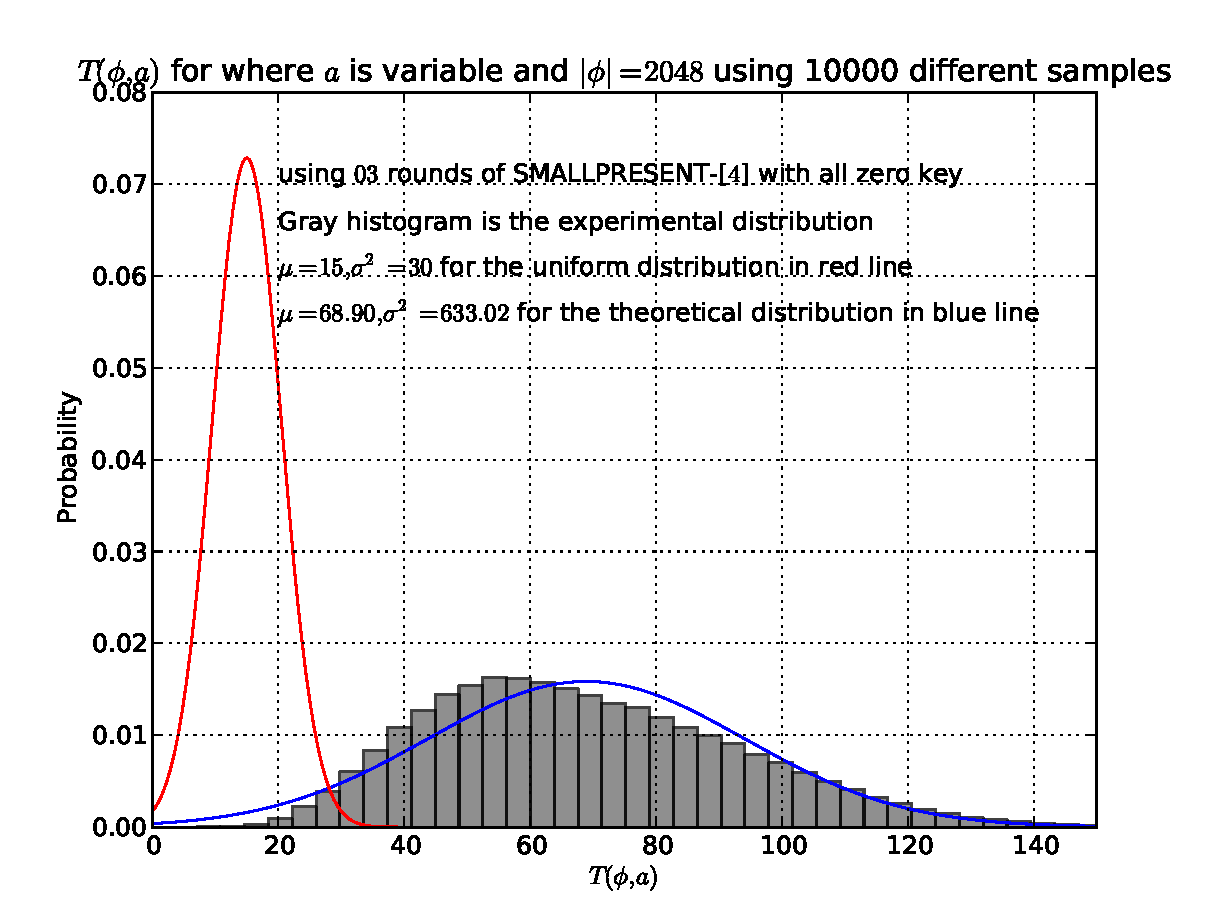
\includegraphics[width= \textwidth , height = 8cm]{images/T_a_phi_variable_a_variable_phi_03_round_plot}
    \caption{$T(\phi,a)$ with $03$ rounds}
    \label{fig:T_a_phi_variable_a_variable_phi_03_round}
\end{figure}
\begin{figure}[h!]
    \centering
    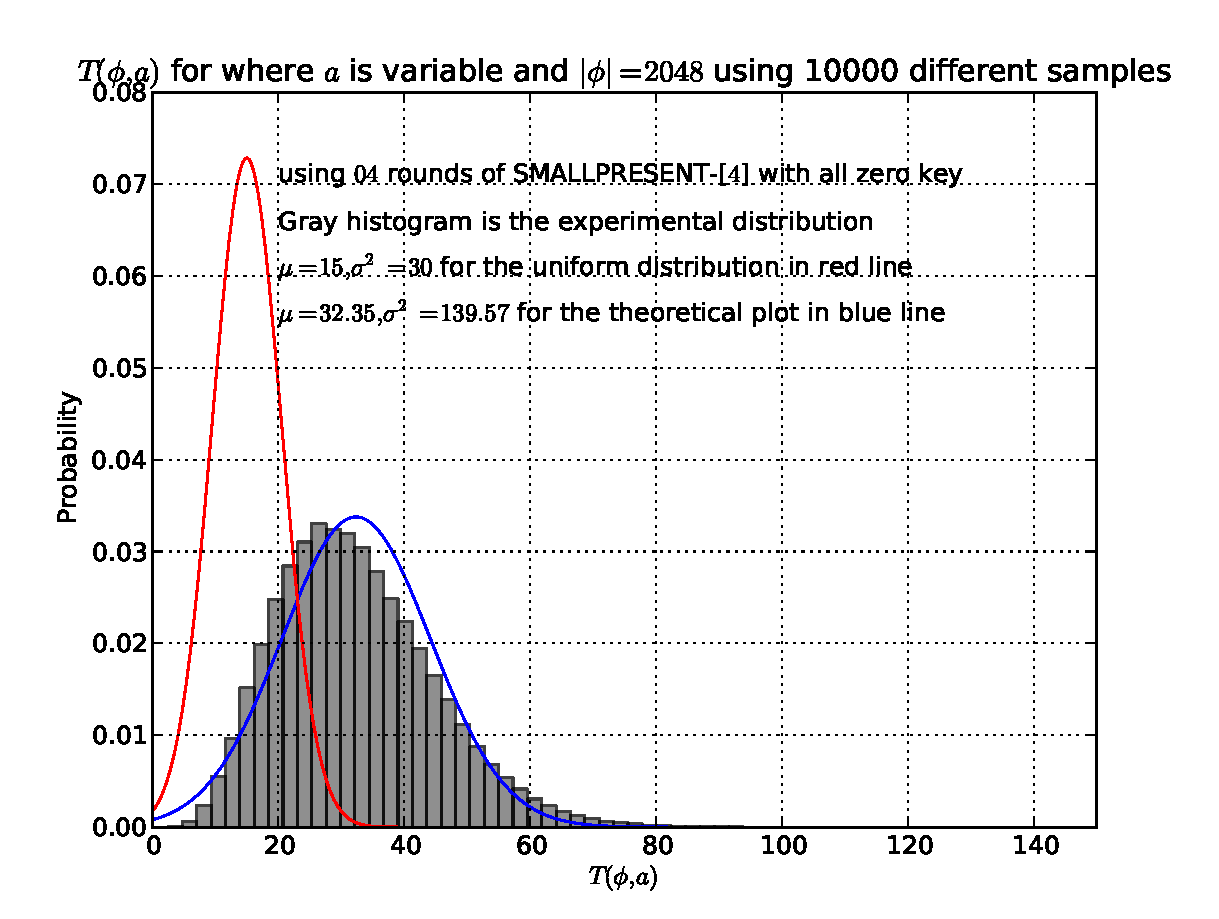
\includegraphics[width=\textwidth , height = 8cm]{images/T_a_phi_variable_a_variable_phi_04_round_plot}
    \caption{$T(\phi,a)$ with $04$ rounds}
    \label{fig:T_a_phi_variable_a_variable_phi_04_round}
\end{figure}

\begin{figure}[h!]
    \centering
    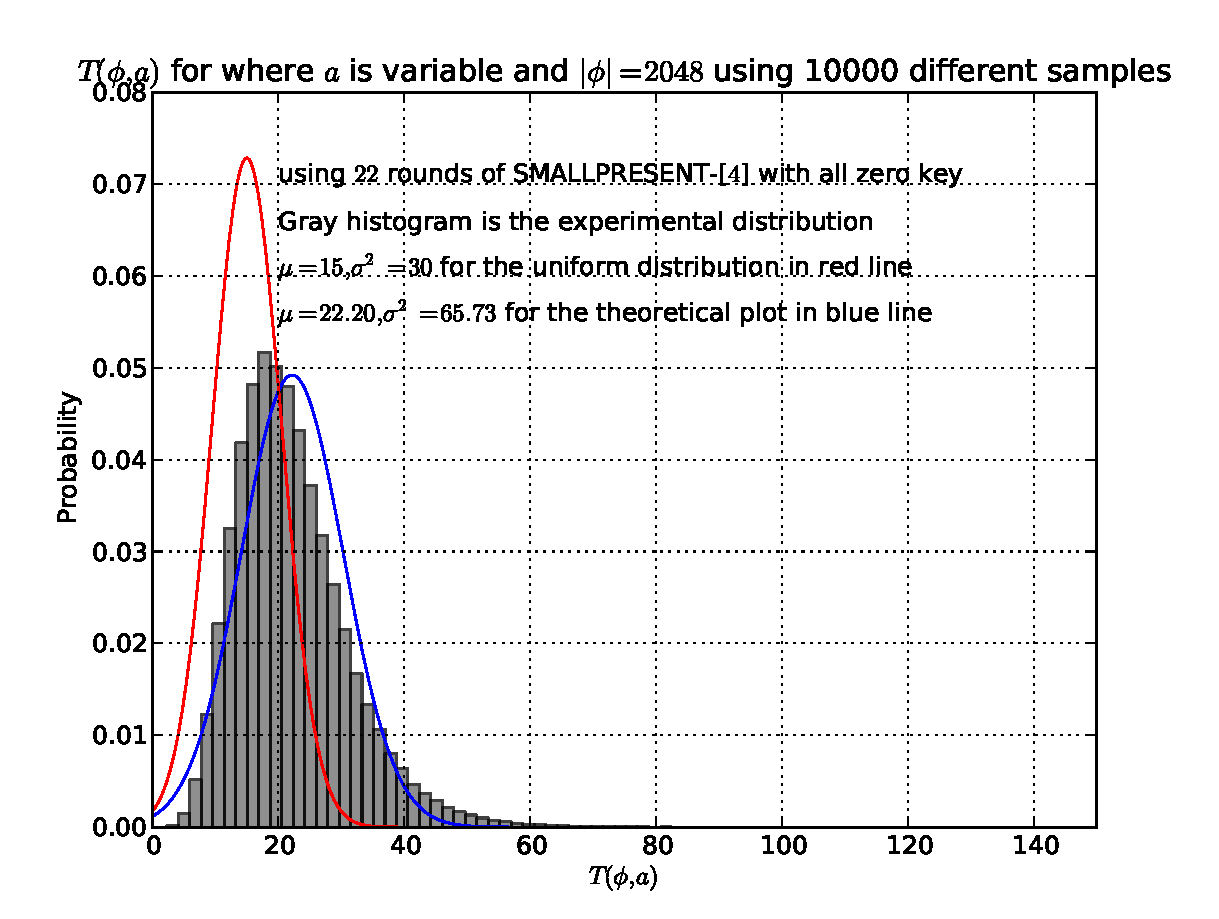
\includegraphics[width=\textwidth , height = 8cm]{images/T_a_phi_variable_a_variable_phi_22_round_plot}
    \caption{$T(\phi,a)$ with $22$ rounds}
    \label{fig:T_a_phi_variable_a_variable_phi_22_round}
\end{figure}

\begin{figure}[h!]
    \centering
    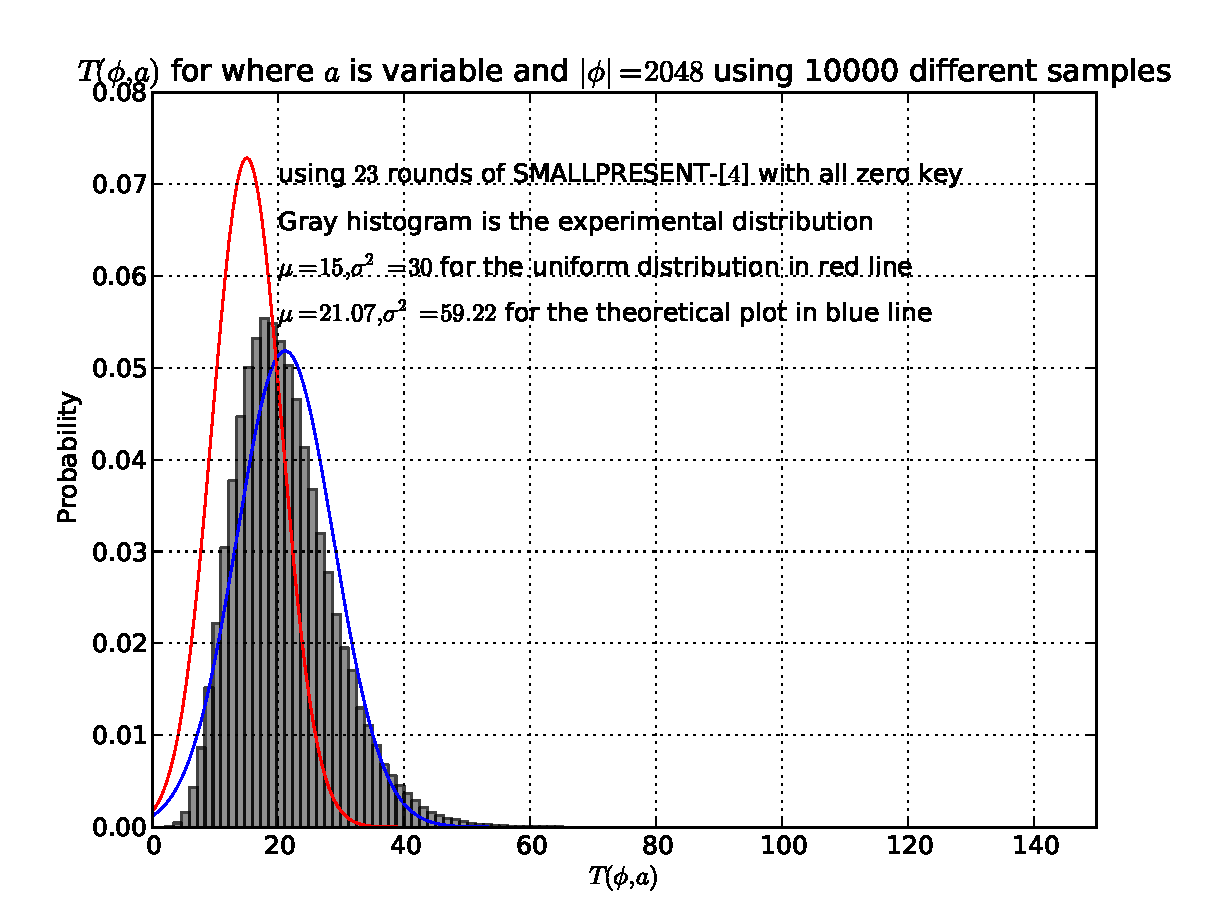
\includegraphics[width=\textwidth , height = 8cm]{images/T_a_phi_variable_a_variable_phi_23_round_plot}
    \caption{$T(\phi,a)$ with $23$ rounds}
    \label{fig:T_a_phi_variable_a_variable_phi_23_round}
\end{figure}

\iffalse

\subsection{Evaluating $T_{a}\left(\phi\right)$ with $\phi$ sampled randomly with replacement:} Here we will be evaluating $T$ for an arbitrarily fixed fixation $a$ or in other words we will now evaluate $T_{a}\left(\phi\right)$ both experimentally and theoretically. We will generate a set $\Phi$ of size $10000$ where each $\phi \in \Phi$ is a randomly chosen (with replacement) subset of  $\mathbb{F}_2^{12}$ and $|\phi| = 2048$. Now for each $\phi \in \Phi$ we will calculate $T_{a}\left(\phi\right)$ according to (\ref{eqn:T_fixed_a_variable_phi}). After that we will calculate the mean and variance of $T_{a}\left(\phi\right)$ over all these $10000$ different $\phi \in \Phi$. And compare this experimentally calculated mean and variance with the theoretically computed mean and variance mentioned in (\ref{eqn:distribution_of_T_fixed_a_variable_phi}). The evaluation is done for $15$ rounds of SMALLPRESENT-$[4]$ and the result is mentioned in Table \ref{table:T_a_phi_fixed_a_variable_fixation}


\begin{center}
\begin{scriptsize}
\captionof{table}{};
\begin{tabular}{l*{4}{c}r} \label{table:T_a_phi_fixed_a_variable_fixation}
$a$ & $\mu_{T_{a}(\phi)}=$ &  $\sigma^2_{T_{a}(\phi)}$ & $C\left(a\right)$ & $\mu_{T_{a}(\phi)}$ & $\sigma^2_{T_{a}(\phi)}$ \\
 & (Experimental) &  (Experimental) &  & (Theoretical) & (Theoretical) \\
\hline
0 & 23.157768 & 64.339134 & 0.004002 & 23.196096 & 62.784384\\
1 & 18.906876 & 45.224827 & 0.001917 & 18.926016 & 45.704064\\
2 & 23.397097 & 63.523018 & 0.004129 & 23.456192 & 63.824768\\
3 & 21.665363 & 56.201130 & 0.003254 & 21.664192 & 57.475968\\
4 & 23.054449 & 61.329144 & 0.003965 & 23.12032 & 62.48128\\
5 & 19.875065 & 49.953552 & 0.002335 & 19.78208 & 49.12832\\
6 & 21.375246 & 55.578331 & 0.003141 & 21.432768 & 55.731072\\
7 & 22.893190 & 60.276630 & 0.003887 & 22.960576 & 61.842304\\
8 & 22.650137 & 62.154163 & 0.003790 & 22.76192 & 61.04768\\
9 & 24.233036 & 63.354294 & 0.004581 & 24.381888 & 67.527552\\
a & 21.359844 & 54.811600 & 0.003134 & 21.418432 & 55.673728\\
b & 17.972765 & 41.687294 & 0.001431 & 17.930688 & 41.722752\\
c & 26.178656 & 74.850182 & 0.005449 & 26.159552 & 74.638208\\
d & 22.964476 & 60.390213 & 0.003950 & 23.0896 & 62.3584\\
e & 19.844593 & 50.031105 & 0.002382 & 19.878336 & 49.513344\\
f & 19.990053 & 50.301014 & 0.002451 & 20.019648 & 50.078592\\
\end{tabular}
\end{scriptsize}
\end{center} \par \noindent Figure \ref{fig:T_a_phi_with_15_rounds_0x00},\ref{fig:T_a_phi_with_15_rounds_0x07}, \ref{fig:T_a_phi_with_15_rounds_0x0b}  shows the distribution of $T_a(\phi)$ for different fixations
\begin{figure}[h!] 
    \centering
    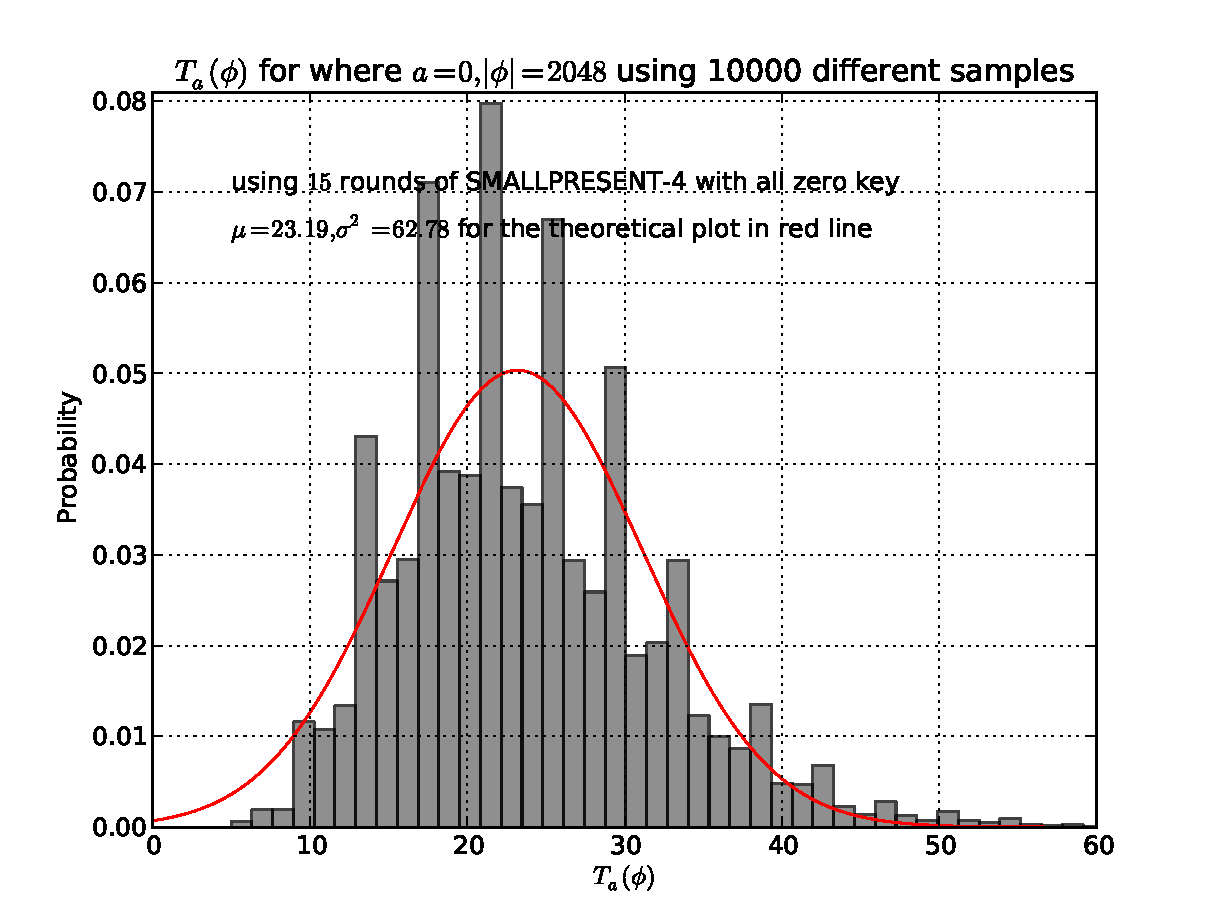
\includegraphics[width=\textwidth , height = 8cm]{images/T_fixed_a_with_value_0_and_variable_phi_size_2048_with_10000_samples}
    \caption{$T_a(\phi)$ with $15$ rounds}
    \label{fig:T_a_phi_with_15_rounds_0x00}
\end{figure}
\begin{figure}[h!]
    \centering
    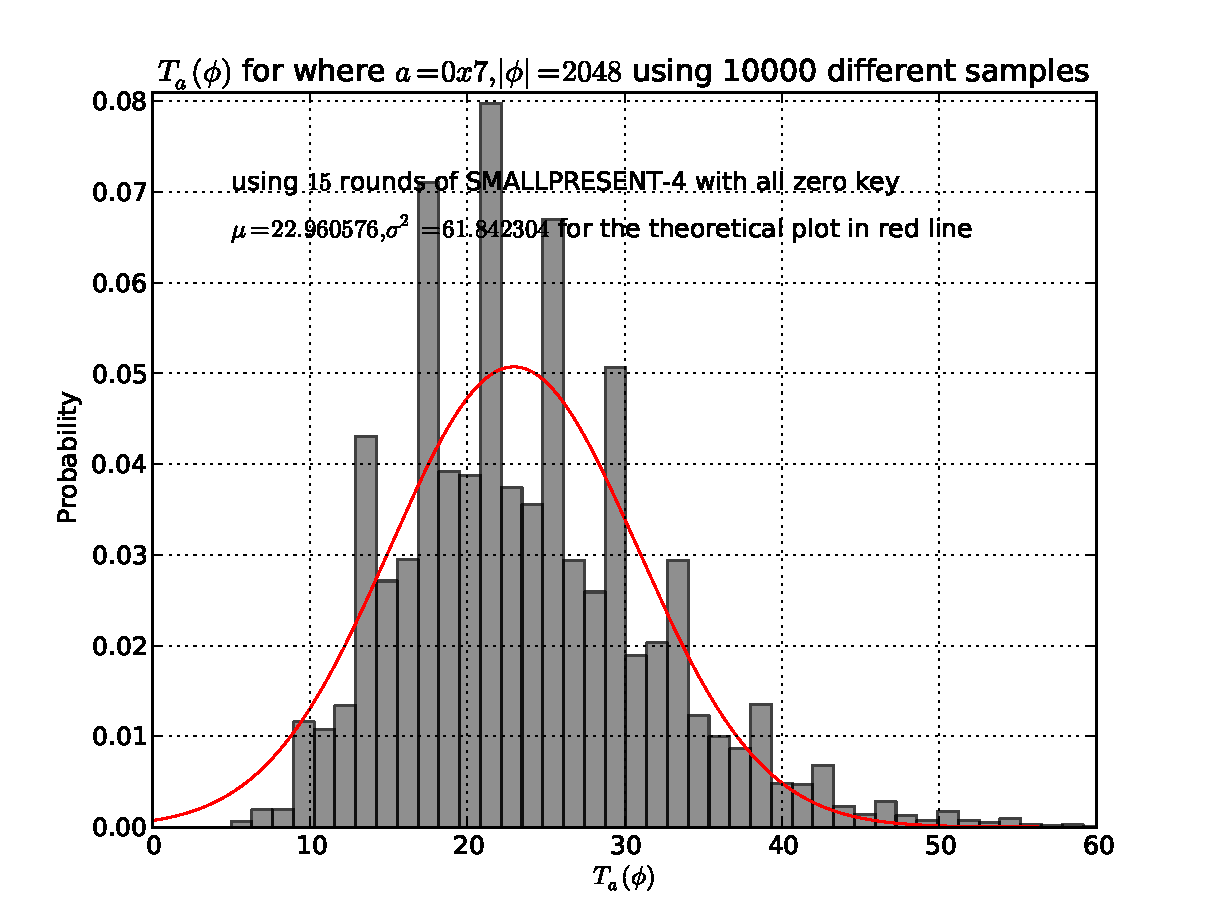
\includegraphics[width=\textwidth , height = 8cm]{images/T_fixed_a_with_value_0x7_and_variable_phi_size_2048_with_10000_samples}
    \caption{$T_a(\phi)$ with $15$ rounds}
    \label{fig:T_a_phi_with_15_rounds_0x07}
\end{figure}
\begin{figure}[h!]
    \centering
    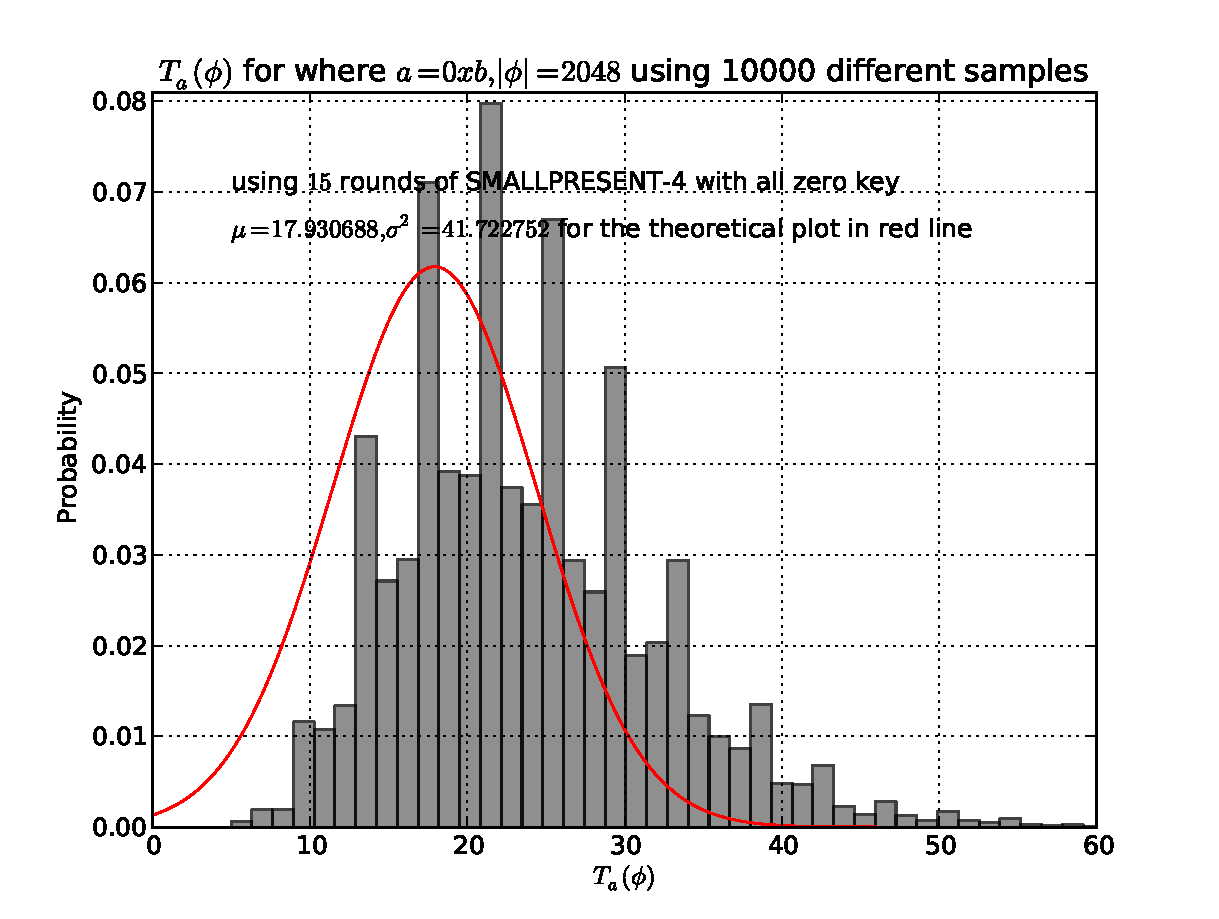
\includegraphics[width=\textwidth , height = 8cm]{images/T_fixed_a_with_value_0xb_and_variable_phi_size_2048_with_10000_samples}
    \caption{$T_a(\phi)$ with $15$ rounds}
    \label{fig:T_a_phi_with_15_rounds_0x0b}
\end{figure} \par \noindent
We observe that there are some spikes in case of a single fixed fixation. But in case variable fixation the theoretical and experimental distribution agrees better.
\fi